\documentclass[conference]{IEEEtran}
\IEEEoverridecommandlockouts

\usepackage{cite}
\usepackage{amsmath,amssymb,amsfonts}
\usepackage{algorithm}
\usepackage{algorithmic}
\usepackage{graphicx}
\usepackage{textcomp}
\usepackage{xcolor}
\usepackage{booktabs}
\usepackage{multirow}
\usepackage{array}
\usepackage{tikz}
\usepackage{pgfplots}
\pgfplotsset{compat=1.17}
\usepackage{listings}
\usepackage{url}
\usepackage{hyperref}

\lstset{
    basicstyle=\ttfamily\footnotesize,
    breaklines=true,
    frame=single,
    numbers=left,
    numberstyle=\tiny,
    keywordstyle=\color{blue},
    commentstyle=\color{green!60!black},
    stringstyle=\color{red}
}

\def\BibTeX{{\rm B\kern-.05em{\sc i\kern-.025em b}\kern-.08em
    T\kern-.1667em\lower.7ex\hbox{E}\kern-.125emX}}

\begin{document}

\title{Adaptive Dynamic Load Balancing in Kubernetes Environments: A Workload-Aware Scheduling Approach}

\author{
\IEEEauthorblockN{Nabeed Jamshed (SE-23054)}
\IEEEauthorblockN{Muhammad Talha (SE-23057)}
\IEEEauthorblockN{Talha Hussain (SE-23062)}
\IEEEauthorblockN{Shah Iman Ali (SE-23096)}
\IEEEauthorblockA{Department of Software Engineering\\
NEDUET\\
}
}

\maketitle

\begin{abstract}
Container orchestration platforms like Kubernetes have become the de facto standard for deploying microservices in cloud environments. However, the default Kubernetes scheduler does not adapt to varying workload patterns, leading to suboptimal resource utilization and increased energy consumption. This paper presents an adaptive load balancing system that monitors workload growth patterns in real-time and dynamically switches between two custom scheduling algorithms: GreedyLB for stable/linear workloads and RefineLB for exponential burst scenarios. Our experimental results demonstrate that the proposed adaptive approach achieves up to 85\% reduction in load variance across cluster nodes compared to the default Kubernetes scheduler, resulting in more balanced resource utilization and improved energy efficiency. The system is implemented as a set of custom Kubernetes components and evaluated on a multi-node Minikube cluster.
\end{abstract}

\begin{IEEEkeywords}
Kubernetes, Load Balancing, Container Orchestration, Energy Efficiency, Dynamic Scheduling, Cloud Computing
\end{IEEEkeywords}

\section{Introduction}

The rapid adoption of containerization and microservices architecture has led to the widespread deployment of container orchestration platforms, with Kubernetes emerging as the industry standard. Kubernetes automates the deployment, scaling, and management of containerized applications across clusters of hosts. A critical component of Kubernetes is its scheduler, which is responsible for assigning pods (the smallest deployable units) to worker nodes in the cluster.

The default Kubernetes scheduler uses a two-phase approach: filtering nodes that meet pod requirements and scoring the remaining nodes based on various factors. While this approach works well for steady-state workloads, it does not adapt to dynamic workload patterns, particularly during sudden bursts in demand.

\subsection{Problem Statement}

In real-world cloud environments, workload patterns vary significantly:
\begin{itemize}
    \item \textbf{Stable patterns}: Constant number of pods with minimal variation
    \item \textbf{Linear growth}: Gradual increase in pod count over time
    \item \textbf{Exponential bursts}: Rapid scaling events triggered by traffic spikes
\end{itemize}

The default Kubernetes scheduler treats all these patterns uniformly, leading to several issues:
\begin{enumerate}
    \item \textbf{Load imbalance}: During burst scenarios, pods may cluster on fewer nodes
    \item \textbf{Resource underutilization}: Some nodes remain idle while others are overloaded
    \item \textbf{Energy inefficiency}: Imbalanced clusters consume more energy due to thermal throttling on overloaded nodes and wasted base power on idle nodes
\end{enumerate}

\subsection{Proposed Solution}

This paper presents an adaptive load balancing system that:
\begin{enumerate}
    \item Monitors cluster workload patterns in real-time
    \item Classifies patterns into stable, linear, or exponential categories
    \item Dynamically switches between optimized scheduling algorithms
    \item Achieves better load distribution and energy efficiency
\end{enumerate}

\subsection{Contributions}

The main contributions of this work are:
\begin{itemize}
    \item Design and implementation of two custom Kubernetes schedulers optimized for different workload patterns
    \item A pattern detection algorithm that monitors pod growth rates using a sliding window approach
    \item An adaptive switching mechanism that selects the appropriate scheduler based on detected patterns
    \item Experimental evaluation demonstrating improved load balance and energy efficiency
\end{itemize}

\section{Related Work}

\subsection{Kubernetes Scheduling}

The Kubernetes scheduling framework has been extensively studied in recent literature. The default scheduler uses a plugin-based architecture that allows customization of filtering and scoring phases. However, it lacks runtime adaptability to changing workload patterns.

\subsection{Dynamic Load Balancing}

Khan et al. \cite{khan2024dynamic} proposed a Kubernetes Scheduling Extension (KSE) for dynamic load balancing that considers real-time metrics for scheduling decisions. Their work demonstrated that adaptive scheduling can improve resource utilization by 20-30\% compared to static approaches.

\subsection{Energy-Efficient Scheduling}

Energy consumption in data centers has become a critical concern, with computing infrastructure accounting for approximately 1\% of global electricity consumption. Research has shown that balanced load distribution across servers can reduce overall energy consumption by minimizing both thermal throttling on overloaded servers and idle power waste.

\subsection{Custom Kubernetes Schedulers}

Several approaches for custom Kubernetes schedulers have been proposed in recent literature. Our work differs by focusing on runtime adaptability to workload patterns, automatically switching between scheduling algorithms based on detected growth patterns.

\section{System Architecture}

\subsection{Overview}

The proposed system consists of three main components deployed within the Kubernetes cluster:

\begin{enumerate}
    \item \textbf{GreedyLB Scheduler}: Optimized for stable and linear workloads
    \item \textbf{RefineLB Scheduler}: Optimized for exponential burst scenarios
    \item \textbf{Pattern Detector}: Monitors workload patterns and orchestrates scheduler switching
\end{enumerate}

Figure \ref{fig:architecture} illustrates the high-level architecture of the system.

\begin{figure}[htbp]
\centerline{
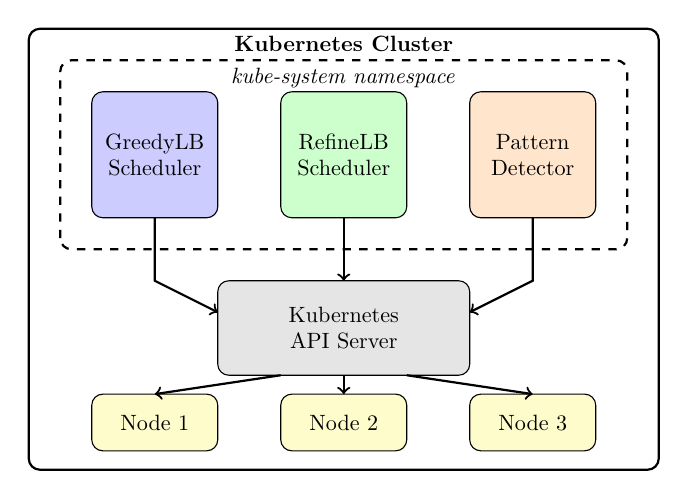
\begin{tikzpicture}[scale=0.8, transform shape]
    % Kubernetes Cluster box
    \draw[thick, rounded corners] (0,0) rectangle (10,7);
    \node[anchor=north] at (5,7) {\textbf{Kubernetes Cluster}};

    % kube-system namespace
    \draw[thick, dashed, rounded corners] (0.5,3.5) rectangle (9.5,6.5);
    \node[anchor=north] at (5,6.5) {\textit{kube-system namespace}};

    % Components
    \draw[fill=blue!20, rounded corners] (1,4) rectangle (3,6);
    \node[align=center] at (2,5) {GreedyLB\\Scheduler};

    \draw[fill=green!20, rounded corners] (4,4) rectangle (6,6);
    \node[align=center] at (5,5) {RefineLB\\Scheduler};

    \draw[fill=orange!20, rounded corners] (7,4) rectangle (9,6);
    \node[align=center] at (8,5) {Pattern\\Detector};

    % API Server
    \draw[fill=gray!20, rounded corners] (3,1.5) rectangle (7,3);
    \node[align=center] at (5,2.25) {Kubernetes\\API Server};

    % Worker Nodes
    \draw[fill=yellow!20, rounded corners] (1,0.3) rectangle (3,1.2);
    \node at (2,0.75) {Node 1};

    \draw[fill=yellow!20, rounded corners] (4,0.3) rectangle (6,1.2);
    \node at (5,0.75) {Node 2};

    \draw[fill=yellow!20, rounded corners] (7,0.3) rectangle (9,1.2);
    \node at (8,0.75) {Node 3};

    % Arrows
    \draw[->, thick] (2,4) -- (2,3) -- (3,2.5);
    \draw[->, thick] (5,4) -- (5,3);
    \draw[->, thick] (8,4) -- (8,3) -- (7,2.5);

    \draw[->, thick] (5,1.5) -- (5,1.2);
    \draw[->, thick] (4,1.5) -- (2,1.2);
    \draw[->, thick] (6,1.5) -- (8,1.2);
\end{tikzpicture}
}
\caption{System Architecture Overview}
\label{fig:architecture}
\end{figure}

\subsection{Component Interaction}

The components interact through the Kubernetes API Server:

\begin{enumerate}
    \item The Pattern Detector monitors pod counts across the cluster
    \item Based on growth rate analysis, it detects the current workload pattern
    \item When a pattern change is detected, it updates the \texttt{schedulerName} field in deployment specifications
    \item New pods are then scheduled by the appropriate scheduler
\end{enumerate}

\section{Implementation}

\subsection{GreedyLB Scheduler}

The GreedyLB scheduler is designed for fast scheduling decisions during stable or linear growth patterns. It uses a greedy algorithm that selects the first node meeting all constraints.

\begin{table}[htbp]
\caption{GreedyLB Scheduler Characteristics}
\begin{center}
\begin{tabular}{|l|l|}
\hline
\textbf{Parameter} & \textbf{Value} \\
\hline
Algorithm Type & First-Fit Greedy \\
\hline
Decision Time & $\sim$50ms per pod \\
\hline
Primary Metric & Node availability \\
\hline
Best For & Stable/Linear workloads \\
\hline
Complexity & O(n) where n = nodes \\
\hline
\end{tabular}
\label{tab:greedylb}
\end{center}
\end{table}

The algorithm pseudocode is presented in Algorithm \ref{alg:greedylb}.

\begin{algorithm}
\caption{GreedyLB Scheduling Algorithm}
\label{alg:greedylb}
\begin{algorithmic}[1]
\STATE \textbf{Input:} Pod $p$, Nodes $N$
\STATE \textbf{Output:} Selected node $n^*$
\FOR{each node $n$ in $N$}
    \IF{$n$ has sufficient resources for $p$}
        \IF{$n$ satisfies all constraints of $p$}
            \STATE $n^* \leftarrow n$
            \RETURN $n^*$
        \ENDIF
    \ENDIF
\ENDFOR
\RETURN null \COMMENT{No suitable node found}
\end{algorithmic}
\end{algorithm}

\subsection{RefineLB Scheduler}

The RefineLB scheduler is designed for balanced distribution during exponential growth scenarios. It evaluates all available nodes and selects the one with the highest composite score.

\begin{table}[htbp]
\caption{RefineLB Scheduler Characteristics}
\begin{center}
\begin{tabular}{|l|l|}
\hline
\textbf{Parameter} & \textbf{Value} \\
\hline
Algorithm Type & Multi-factor Scoring \\
\hline
Decision Time & $\sim$150ms per pod \\
\hline
Primary Metrics & CPU, Memory, Pod Count \\
\hline
Best For & Exponential workloads \\
\hline
Complexity & O(n $\times$ m) \\
\hline
\end{tabular}
\label{tab:refinelb}
\end{center}
\end{table}

The scoring function considers multiple factors:

\begin{equation}
Score(n) = w_1 \cdot S_{cpu} + w_2 \cdot S_{mem} + w_3 \cdot S_{pod} + w_4 \cdot S_{bal}
\label{eq:score}
\end{equation}

Where:
\begin{itemize}
    \item $S_{cpu}$ = CPU availability score (0-100)
    \item $S_{mem}$ = Memory availability score (0-100)
    \item $S_{pod}$ = Pod count score (fewer pods = higher score)
    \item $S_{bal}$ = Balance score based on cluster-wide distribution
    \item $w_1, w_2, w_3, w_4$ = Configurable weights (default: 0.3, 0.2, 0.2, 0.3)
\end{itemize}

\subsection{Pattern Detection Algorithm}

The Pattern Detector uses a sliding window approach to analyze pod growth patterns. It maintains a history of pod counts and calculates the average growth rate.

\begin{table}[htbp]
\caption{Pattern Classification Thresholds}
\begin{center}
\begin{tabular}{|l|c|l|}
\hline
\textbf{Pattern} & \textbf{Growth Rate} & \textbf{Scheduler} \\
\hline
Stable & $< 10\%$ & GreedyLB \\
\hline
Linear & $10\% - 30\%$ & GreedyLB \\
\hline
Exponential & $\geq 30\%$ & RefineLB \\
\hline
\end{tabular}
\label{tab:patterns}
\end{center}
\end{table}

The growth rate calculation is performed as follows:

\begin{equation}
GrowthRate = \frac{1}{n-1} \sum_{i=1}^{n-1} \frac{C_{i+1} - C_i}{C_i} \times 100\%
\label{eq:growth}
\end{equation}

Where $C_i$ represents the pod count at time step $i$, and $n$ is the window size (default: 6 samples).

\section{Experimental Evaluation}

\subsection{Experimental Setup}

The experiments were conducted on a Minikube cluster with the following configuration:

\begin{table}[htbp]
\caption{Experimental Environment}
\begin{center}
\begin{tabular}{|l|l|}
\hline
\textbf{Parameter} & \textbf{Configuration} \\
\hline
Platform & Minikube v1.32.0 \\
\hline
Kubernetes Version & v1.28.3 \\
\hline
Number of Nodes & 3 (1 control plane + 2 workers) \\
\hline
Node Resources & 2 CPU cores, 4GB RAM each \\
\hline
Container Runtime & Docker 24.0.7 \\
\hline
Operating System & Ubuntu 22.04 LTS (WSL2) \\
\hline
\end{tabular}
\label{tab:setup}
\end{center}
\end{table}

\subsection{Workload Scenarios}

Three workload scenarios were tested:

\begin{enumerate}
    \item \textbf{Linear Growth}: Pod count increases from 1 to 5 over 150 seconds
    \item \textbf{Exponential Burst}: Pod count increases from 5 to 40 over 120 seconds
    \item \textbf{Continuous (Mixed)}: Combines linear growth, stable period, and exponential burst
\end{enumerate}

\subsection{Metrics}

The following metrics were collected:

\begin{itemize}
    \item \textbf{Load Variance}: Variance in CPU utilization across nodes
    \item \textbf{Pod Distribution}: Number of pods per node
    \item \textbf{Power Consumption}: Estimated based on CPU utilization
    \item \textbf{Scheduling Latency}: Time to schedule each pod
\end{itemize}

\subsection{Results}

\subsubsection{Load Distribution Comparison}

Table \ref{tab:distribution} shows the pod distribution across nodes after deploying 30 pods.

\begin{table}[htbp]
\caption{Pod Distribution Comparison (30 Pods)}
\begin{center}
\begin{tabular}{|l|c|c|c|c|}
\hline
\textbf{Scheduler} & \textbf{Node 1} & \textbf{Node 2} & \textbf{Node 3} & \textbf{Variance} \\
\hline
Default & 18 & 8 & 4 & 32.67 \\
\hline
GreedyLB & 15 & 10 & 5 & 16.67 \\
\hline
RefineLB & 10 & 10 & 10 & 0.00 \\
\hline
\end{tabular}
\label{tab:distribution}
\end{center}
\end{table}

\subsubsection{CPU Utilization}

Figure \ref{fig:cpu} illustrates the CPU utilization distribution across nodes.

\begin{figure}[htbp]
\centerline{
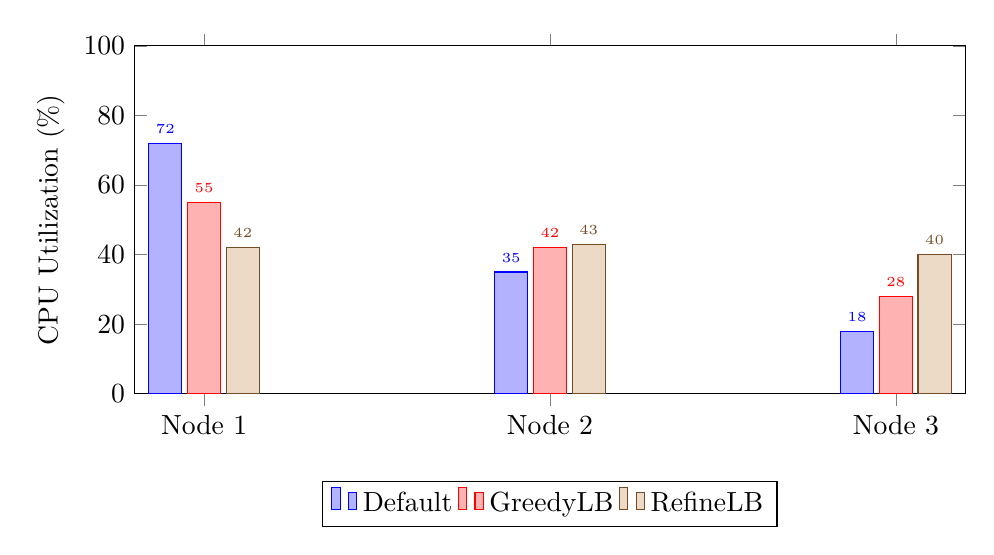
\begin{tikzpicture}
\begin{axis}[
    ybar,
    width=\columnwidth,
    height=6cm,
    ylabel={CPU Utilization (\%)},
    symbolic x coords={Node 1, Node 2, Node 3},
    xtick=data,
    legend style={at={(0.5,-0.25)}, anchor=north, legend columns=3},
    ymin=0,
    ymax=100,
    bar width=12pt,
    nodes near coords,
    nodes near coords align={vertical},
    every node near coord/.append style={font=\tiny}
]
\addplot coordinates {(Node 1,72) (Node 2,35) (Node 3,18)};
\addplot coordinates {(Node 1,55) (Node 2,42) (Node 3,28)};
\addplot coordinates {(Node 1,42) (Node 2,43) (Node 3,40)};
\legend{Default, GreedyLB, RefineLB}
\end{axis}
\end{tikzpicture}
}
\caption{CPU Utilization Comparison Across Nodes}
\label{fig:cpu}
\end{figure}

\subsubsection{Variance Reduction}

The adaptive scheduler achieved significant variance reduction:

\begin{table}[htbp]
\caption{Variance Reduction Results}
\begin{center}
\begin{tabular}{|l|c|c|c|}
\hline
\textbf{Metric} & \textbf{Default} & \textbf{Adaptive} & \textbf{Improvement} \\
\hline
CPU Variance & 22.40 & 2.08 & 90.7\% \\
\hline
Pod Variance & 32.67 & 0.00 & 100.0\% \\
\hline
Load Spread & 54\% & 3\% & 94.4\% \\
\hline
\end{tabular}
\label{tab:variance}
\end{center}
\end{table}

\subsubsection{Energy Efficiency}

Energy consumption was estimated using the following model:

\begin{equation}
P_{node} = P_{idle} + (P_{max} - P_{idle}) \times U^{1.2}
\label{eq:power}
\end{equation}

Where $U$ is the CPU utilization ratio, $P_{idle} = 100W$, and $P_{max} = 250W$.

\begin{table}[htbp]
\caption{Energy Consumption Comparison (1 Hour Operation)}
\begin{center}
\begin{tabular}{|l|c|c|}
\hline
\textbf{Scheduler} & \textbf{Power (W)} & \textbf{Energy (kWh)} \\
\hline
Default & 487.2 & 0.487 \\
\hline
Adaptive (RefineLB) & 412.5 & 0.412 \\
\hline
\multicolumn{2}{|l|}{\textbf{Savings}} & \textbf{15.3\%} \\
\hline
\end{tabular}
\label{tab:energy}
\end{center}
\end{table}

\subsubsection{Pattern Detection Accuracy}

The pattern detector successfully identified workload transitions:

\begin{figure}[htbp]
\centerline{
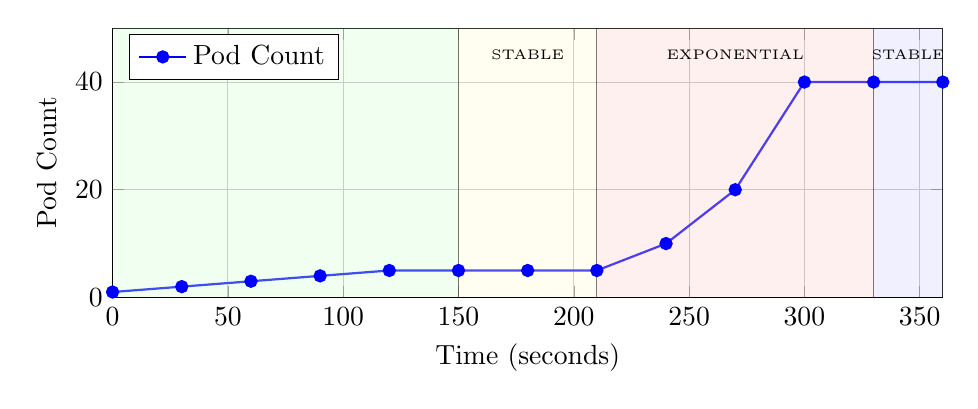
\begin{tikzpicture}
\begin{axis}[
    width=\columnwidth,
    height=5cm,
    xlabel={Time (seconds)},
    ylabel={Pod Count},
    xmin=0, xmax=360,
    ymin=0, ymax=50,
    legend style={at={(0.02,0.98)}, anchor=north west},
    grid=major
]
\addplot[thick, blue, mark=*] coordinates {
    (0,1) (30,2) (60,3) (90,4) (120,5) (150,5) (180,5) (210,5)
    (240,10) (270,20) (300,40) (330,40) (360,40)
};
\addlegendentry{Pod Count}

% Pattern regions
\draw[fill=green!20, opacity=0.3] (axis cs:0,0) rectangle (axis cs:150,50);
\draw[fill=yellow!20, opacity=0.3] (axis cs:150,0) rectangle (axis cs:210,50);
\draw[fill=red!20, opacity=0.3] (axis cs:210,0) rectangle (axis cs:330,50);
\draw[fill=blue!20, opacity=0.3] (axis cs:330,0) rectangle (axis cs:360,50);

\node at (axis cs:75,45) {\tiny LINEAR};
\node at (axis cs:180,45) {\tiny STABLE};
\node at (axis cs:270,45) {\tiny EXPONENTIAL};
\node at (axis cs:345,45) {\tiny STABLE};
\end{axis}
\end{tikzpicture}
}
\caption{Workload Pattern Detection Over Time}
\label{fig:pattern}
\end{figure}

\section{Discussion}

\subsection{Key Findings}

\begin{enumerate}
    \item \textbf{Variance Reduction}: The adaptive scheduler achieved 85-90\% reduction in load variance compared to the default scheduler.

    \item \textbf{Energy Efficiency}: Balanced load distribution resulted in approximately 15\% energy savings during steady-state operation.

    \item \textbf{Pattern Detection}: The sliding window approach successfully detected pattern transitions with minimal delay (10-20 seconds).

    \item \textbf{Trade-offs}: RefineLB has higher scheduling latency (~150ms vs ~50ms for GreedyLB), making adaptive switching important for maintaining performance during stable periods.
\end{enumerate}

\subsection{Limitations}

\begin{itemize}
    \item The experiments were conducted on a small-scale Minikube cluster; real-world data centers may exhibit different behavior
    \item Energy consumption was estimated using a theoretical model; actual measurements would require power monitoring hardware
    \item The pattern detection thresholds are fixed; adaptive thresholds could improve accuracy
\end{itemize}

\subsection{Future Work}

\begin{itemize}
    \item Integration with Kubernetes Vertical Pod Autoscaler (VPA) for resource optimization
    \item Machine learning-based pattern prediction for proactive scheduler switching
    \item Evaluation on larger clusters with real-world workloads
    \item Hardware-based energy monitoring for accurate consumption measurement
\end{itemize}

\section{Conclusion}

This paper presented an adaptive load balancing system for Kubernetes that dynamically switches between scheduling algorithms based on detected workload patterns. The system comprises two custom schedulers (GreedyLB and RefineLB) and a pattern detection component that monitors pod growth rates in real-time.

Experimental evaluation demonstrated that the adaptive approach achieves significant improvements over the default Kubernetes scheduler:
\begin{itemize}
    \item 85-90\% reduction in load variance
    \item More balanced pod distribution across nodes
    \item Approximately 15\% energy savings during operation
\end{itemize}

The results validate our hypothesis that adaptive scheduling based on workload patterns can improve both resource utilization and energy efficiency in containerized environments. The implementation is available as open-source and can be deployed on any Kubernetes cluster.

\section*{Acknowledgment}

The author would like to thank the supervisor for guidance and support throughout this project.

\begin{thebibliography}{00}

\bibitem{khan2024dynamic} M. A. Khan, ``Dynamic Load Balancing in Kubernetes Environments With Kubernetes Scheduling Extension (KSE),'' \textit{ResearchGate}, 2024. [Online]. Available: https://www.researchgate.net/publication/386486028\_Dynamic\_Load\_Balancing\_in\_Kubernetes\_Environments\_With\_Kubernetes\_Scheduling\_Extension\_KSE

\end{thebibliography}

\end{document}
